\documentclass[tikz,border=10pt]{standalone}
\usepackage{pgf}
\usepackage{xcolor}

\begin{document}
	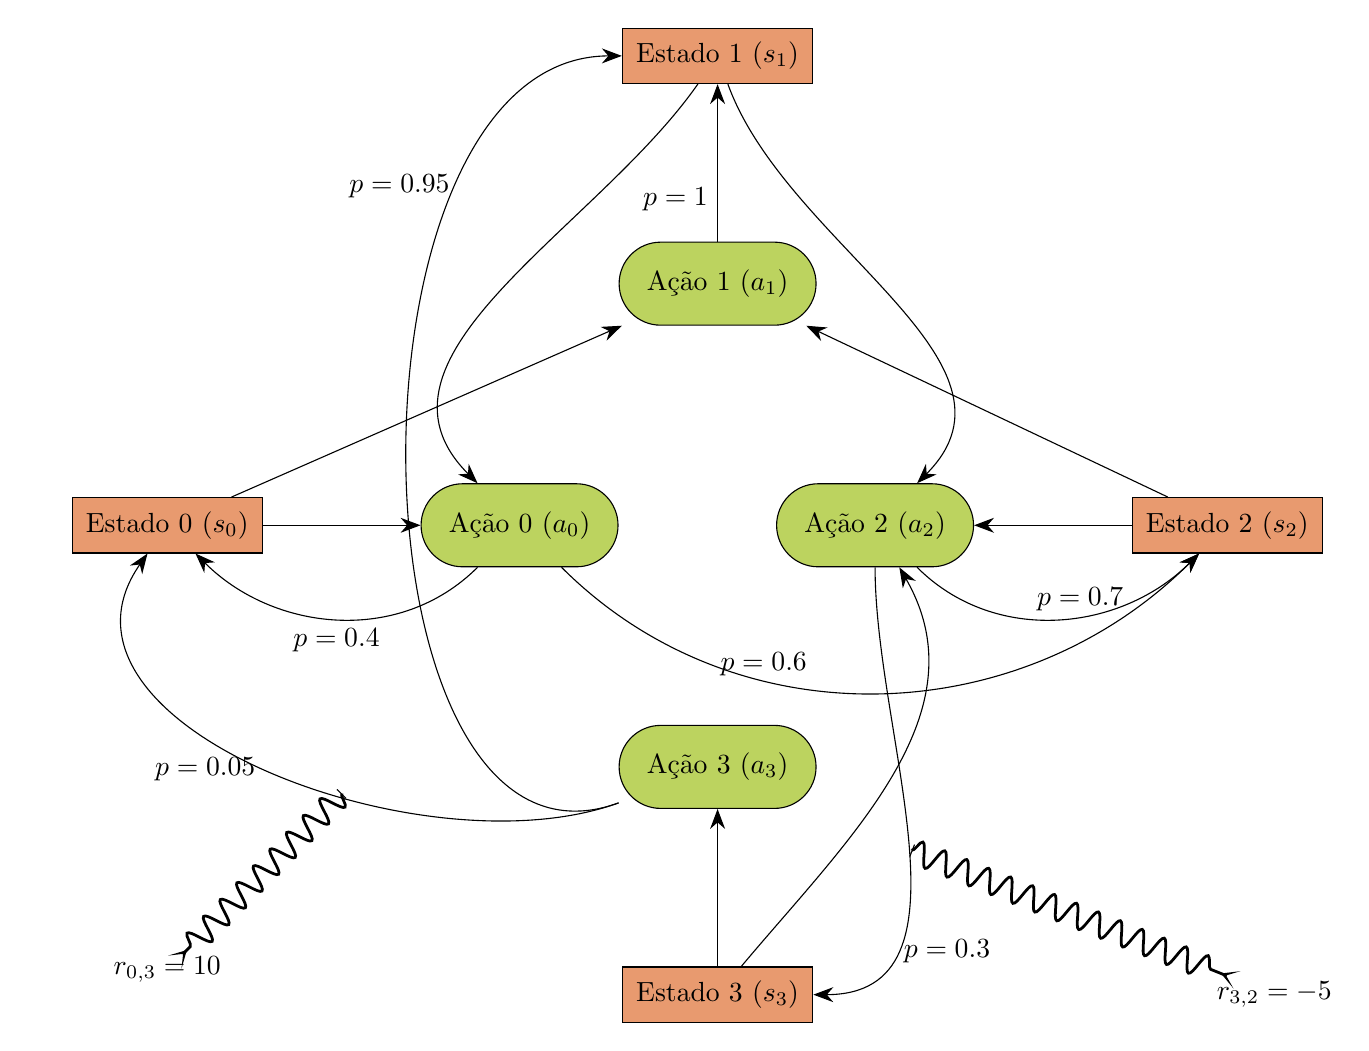
\begin{tikzpicture}
		\usetikzlibrary{arrows,automata,positioning,arrows.meta};
		\definecolor{statecolor}{HTML}{e89a6f};
		\definecolor{actioncolor}{HTML}{bcd35f};
		\tikzset{
			state/.style={
				shape=rectangle,
				draw=black,
				fill=statecolor,
				align=center,
				minimum height=2em,
				minimum width=4em,
				inner sep=5pt,
			},
			action/.style={
				shape=rectangle,
				draw=black,
				fill=actioncolor,
				align=center,
				inner sep=10pt,
				rounded corners=15pt,
			},
			reward/.style={
				|-,
				decoration={snake, amplitude=1.5mm, segment length=3mm},
				decorate,
				postaction={draw, line width=1pt, -{Stealth[scale=-0.8]}}
			},
			transition/.style={
				->,
				>={Stealth[scale=1.5]},
			}
		};
		\tikzset{node distance=2cm and 2cm}
    	\node[state] (s0) {Estado 0 ($s_0$)};

		\node[action, right=2cm of s0] (a0) {Ação 0 ($a_0$)};
		\node[action, above right=2cm and 0cm of a0] (a1) {Ação 1 ($a_1$)};
		\node[action, right=2cm of a0] (a2) {Ação 2 ($a_2$)};
		\node[action, below right=2cm and 0cm of a0] (a3) {Ação 3 ($a_3$)};

		\node[state, above=2cm of a1] (s1) {Estado 1 ($s_1$)};
		\node[state, right=2cm of a2] (s2) {Estado 2 ($s_2$)};
		\node[state, below=2cm of a3] (s3) {Estado 3 ($s_3$)};
		
		\node[draw=none, below right=2.8cm and 1cm of s0] (r0s) {};
		\node[draw=none, below=5cm of s0] (r0e) {$r_{0, 3}=10$};
		
		\node[draw=none, above right=1.4cm and 1cm of s3] (r1s) {};
		\node[draw=none, right=5cm of s3] (r1e) {$r_{3, 2}=-5$};
		
		\begin{scope} % actions
			\draw[transition] 
			(s0) 
			to
			(a0);
	
			\draw[transition] 
			(s0) 
			to
			(a1);
	
			\draw[transition] 
			(s1) 
			to[in=45, out=290]
			(a2);
	
			\draw[transition] 
			(s1) 
			to[in=135, out=235]
			(a0);
	
			\draw[transition] 
			(s2) 
			to
			(a1);
	
			\draw[transition] 
			(s2) 
			to
			(a2);
	
			\draw[transition] 
			(s3) 
			to
			(a3);
	
			\draw[transition] 
			(s3) 
			to[in=300, out=50]
			(a2);		
		\end{scope}
		
		\begin{scope} % transitions
			\draw[transition] 
			(a0)
			to[in=315, out=225] node[midway, below] 
			{$p = 0.4$} 
			(s0);
			
			\draw[transition] 
			(a0) 
			to[in=225, out=315] node[near start, right] 
			{$p = 0.6$} 
			(s2);
			
			\draw[transition] 
			(a1) 
			to[in=270, out=90] node[near start, left] 
			{$p = 1$} 
			(s1);
			
			\draw[transition] 
			(a2) 
			to[in=225, out=315] node[near end, left] 
			{$p = 0.7$} 
			(s2);
			
			\draw[transition] 
			(a2) 
			to[in=0, out=270] node[near end, right] 
			{$p = 0.3$} 
			(s3);
			
			\draw[transition] 
			(a3) 
			to[in=235, out=200] node[midway, left] 
			{$p = 0.05$} 
			(s0);
			
			\draw[transition] 
			(a3) 
			to[in=180, out=200] node[near end, left] 
			{$p = 0.95$} 
			(s1);
		\end{scope}
		
		\begin{scope}
			\draw[reward]
			(r0s)
			to
			(r0e);
			
			\draw[reward]
			(r1s)
			to
			(r1e);
			
		\end{scope}
	\end{tikzpicture}
\end{document}
